\documentclass[a4paper,10pt,reqno,oneside]{amsart}
\usepackage[small]{caption}
%\usepackage[usenames,dvipsnames]{color}
%\usepackage[colorlinks=TRUE,linkcolor=Black,urlcolor=Black,citecolor=Black,pagebackref=TRUE,]{hyperref} %Have to change href email.
\usepackage{amsfonts,fancyhdr,graphicx,lastpage,rotating,multirow,fixltx2e, stfloats,txfonts,palatino,url,xcolor,multicol,hanging, setspace,lscape, paralist, changepage,subcaption,array,verbatim,setspace, siunitx, tikz, flafter}
\usepackage[pagewise,displaymath, mathlines]{lineno}
\usepackage{epstopdf}
\renewcommand{\theequation}{eqn \arabic{equation}}
\makeatletter
\def\tagform@#1{\maketag@@@{\ignorespaces#1\unskip\@@italiccorr}}
\makeatother



\usepackage[nolists, nomarkers, tablesfirst]{endfloat}
\linenumbers
\doublespacing

\usepackage[compress,semicolon]{natbib}



% This declares the unit "animals". Also redefined days to be whole word *(not sure if thats what is needed.
\DeclareSIUnit{\animals}{animals}
\DeclareSIUnit{\day}{days}







\definecolor{approachCol}{rgb}{0.96,0.96,0.96}


\newcommand{\segment}[2]{
	\draw[ultra thick] (0,0) -- ++(90-#1/2:#2cm)
     	      (0,0) -- ++(90+#1/2:#2cm);
	\draw[ultra thick] (0,0) ++(90-#1/2:#2cm) arc (90-#1/2:90+#1/2:#2cm);
}


\newcommand{\profilextwo}[3]{ % angle, sensor width, r
	\draw[ultra thick, red] ({#3*cos(90-#2/2)}, {#3*sin(90-#2/2)}) 
	--++ (270-#1: {2*#3*sin(#2/2)*sin(#1)});
}

\newcommand{\profilexthree}[3]{ % angle, sensor width, r
	\draw[ultra thick, red] ({#3*cos(90-#2/2)}, {#3*sin(90-#2/2)}) 
	--++ (180-#2/2+#1: {#3*sin(#1)});
}



\newcommand{\approachtwo}[4]{ % angle, sensor width, r
	\fill[ approachCol] ({#3*cos(90-#2/2)}, {#3*sin(90-#2/2)}) 
	--++ (180-#1: #4/2)
	--++ (270-#1: {2*#3*sin(#2/2)*sin(#1)}) 
	--++ (360-#1: #4)
	--++ (90-#1: {2*#3*sin(#2/2)*sin(#1)})
	-- cycle;
	\fill[ approachCol ] ({#3*cos(90-#2/2)+1.1*#4*sin(90-#1)/2}, {#3*sin(90-#2/2)-1.1*#4*cos(90-#1)/2}) 
	--++ (270-#1: {2*#3*sin(#2/2)*sin(#1)})
	--++ (-15-#1+90: {#3*sin(#2/2)*sin(#1)/cos(15)})
	-- cycle;
}





\begin{document}


\title[A generalised random encounter model for animals]{A generalised random encounter model for estimating animal density with remote sensor data}
\maketitle

\subsection*{ Running title: A generalised random encounter model for animals}

\subsection*{ Word count:}

\subsection*{ Authors:\\}
Tim C.D. Lucas\textsuperscript{1,2,3}, Elizabeth A. Moorcroft\textsuperscript{1,4,5}, Robin Freeman\textsuperscript{5}, Marcus J. Rowcliffe\textsuperscript{5}, Kate E. Jones\textsuperscript{2,5}


\subsection*{ Addresses:\\}
1 CoMPLEX, University College London, Physics Building, Gower Street, London, WC1E 6BT, UK\\ 
2 Centre for Biodiversity and Environment Research, Department of Genetics, Evolution and Environment, University College London, Gower Street, London, WC1E 6BT, UK\\ 
3 Department of Statistical Science, University College London, Gower Street, London, WC1E 6BT, UK\\ 
4 Department of Computer Science, University College London, Gower Street, London, WC1E 6BT, UK\\ 
5 Institute of Zoology, Zoological Society of London, Regents Park, London, NW1 4RY, UK


\subsection*{ Corresponding authors:\\}
Kate E. Jones,\\
Centre for Biodiversity and Environment Research,\\
Department of Genetics, Evolution and Environment,\\
University College London,\\
Gower Street,\\
London,\\
WC1E 6BT, \\
UK\\
kate.e.jones@ucl.ac.uk\\

Marcus J. Rowcliffe, \\
Institute of Zoology, \\
Zoological Society of London, \\
Regents Park, \\
London, \\
NW1 4RY, \\
UK \\
marcus.rowcliffe@ioz.ac.uk


\clearpage


%max word count 350 words. - current count 347

\section{Abstract}
\subsection*{1:}  Wildlife monitoring technology has advanced rapidly and the use of remote sensors such as camera traps, and acoustic detectors is becoming common in both the terrestrial and marine environments. Current capture-recapture or distance methods to estimate abundance or density require individual recognition of animals or knowing the distance of the animal from the sensor, which is often difficult. A method without these requirements, the random encounter model (REM), has been successfully applied to estimate animal densities from count data generated from camera traps. However, count data from acoustic detectors do not fit the assumptions of the REM due to the directionality of animal signals.

\subsection*{2:} We developed a generalised REM (gREM), to estimate absolute animal density from count data from both camera traps and acoustic detectors. We derived the gREM for different combinations of sensor detection widths and animal signal widths (a measure of directionality). We tested the accuracy and precision of this model using simulations of different combinations of sensor detection widths and animal signal widths, number of captures, and models of animal movement. 

\subsection*{3:} We find that the gREM produces accurate estimates of absolute animal density for all combinations of sensor detection widths and animal signal widths. However, larger sensor detection and animal signal widths were found to be more precise. While the model is accurate for all capture efforts tested, the precision of the estimate increases with the number of captures. We found no effect of different animal movement models tested on the accuracy and precision of the gREM.  

\subsection*{4:} We conclude that the gREM provides an effective method to estimate absolute animal densities from remote sensor count data over a range of sensor and animal signal widths. The gREM is applicable for use for count data obtained in both marine and terrestrial environments, visually or acoustically (e.g., big cats, sharks, birds, bats and cetaceans). As sensors such as camera traps and acoustic detectors become more ubiquitous, the gREM will be increasingly useful for monitoring animal populations across broad spatial, temporal and taxonomic scales. 

\subsection{Keywords} %max keywords/phrase 10 - current 3
Acoustic detection, Camera traps, Marine, Population monitoring, Simulations, Terrestrial 

\section{Introduction}

Wildlife montoring important (declines in populations, global declines)
Wildlife monitoring tech growing in sophication and widespread (remote sensors visual and acoustic)
Difficult to estimate abundance and densities (needed for monitoring)
Current methods are often inadequate because of specific data requirements (marked indivudals)
REM developed for camera trap data, doesnt need this assumptions 
but has limitations
Specifically sensor widths - different environments might need more flexibility (examples) and signal directionality assumptions (examples) - method has been optimised for terrestrial large animals
acoustic monitoring becoming more common method of monitoring but has additional sensor width problems (examples) and directionality of signals (examples). 
Currently the count data from acoustic monitoring is used for monitoring in different ways (examples). 
Another limitation to using these sensors is lack of guidelines on how survey effort impacts the accuracy and precision of estimates (guidelines would be useful. practically can only be done within simulated environment, rarely done)
We develop gREM and tested it and come up with specific recommedations for its use (providing code for implementation). we controlled for different animal movement by testing the robustness of gREM with different movement model (examples).

Animal population size is one of the fundamental measures needed in ecology and conservation. The absolute size of a population has important implications for a range of issues such as genetic diversity \citep{o1985genetic, fischer2000genetic, willi2005threefold}, sensitivity to stochastic fluctuations \citep{richter1972extinction,wright1983stochastic} and risk of extinction \citep{purvis2000predicting}. Sensor technology, such as camera traps \citep{rowcliffe2008surveys,ahumada2011community} and acoustic detectors \citep{ofarrel1999comparison,mellinger2007fixed,jones2011indicator} are becoming increasingly used to survey animal populations, as they are efficient, relativity cheap and non-invasive \citep{gese2001monitoring, o2003crouching, silveira2003camera}, allowing for surveys over large areas and long periods. 

However, the problem of converting sampled count data to estimates of density remains. The preferred method for estimating density if individuals can be recognised is capture-recapture e.g. \citep{karanth1995, trolle2003estimation, soisalo2006estimating, trolle2007camera}. If individual recognition is impossible but the distance between animal and sensor can be estimated, distance sampling methods can be used to estimate density, although these often ignore animal movement which may bias estimates \citep{barlow2005estimates, marques2011estimating}. Finally, methods for density estimation, based on ideal gas models (originally formulated by physicists to estimate contact rates between molecules) have been developed \citep{yapp1956theory, Hutchinson_Waser_2007}. The gas model has been modified for use with camera traps, which have an angle of detection (the angle within which an animal can be detected)  up to $\pi$ radians \citep{rowcliffe2008estimating}. This angle limitation may not apply to acoustic sensors. Furthermore, animal calls may be directional, and the existing random encounter model (REM) designed for camera trap data does not handle this case.

%Some species are much more easily detected or identified by acoustic detectors. For example, while bat identification by hand requires much training, methods are being developed to automatically identify species from their calls \citep{Adams_2010,walters_2012}. With respect to distance (or the radius of detection), large Cetaceans are loud enough to detected from tens of kilometres away, further than is possible visually \citep{clark1995application, mcdonald2004difar,barlow2005estimates}.  

%However, many authors highlight the need to consider detectability when estimating density, since failure to do so will usually give biased results. In particular, this bias has been highlighted as a problem for the interpretation of count rates from sensors such as camera traps \citep{jennelle2002use, foster2012critique}.

In this study we create a generalised REM (gREM), as an extension to the camera trap model of \citep{rowcliffe2008estimating}, to estimate absolute density from count data from acoustic detectors, or camera traps, where the sensor angle can vary from 0 to $2\pi$ radians, and the acoustic signal given off from the animal can be directional (we call the width of an animals acoustic call the call angle).  We tested the model using simulations in order to assess the validity of the models and in order to give suggestions for best practice. Specifically, we test that the analytical model can accurately predict density when the assumptions of a homogeneous environment and straight-line animal movement are met. We went on to test the accuracy of the model if the assumptions about animal movement were broken, including non-continuous movement and correlated and random walks. 

\section{Methods}

\subsection{Analytical Model}

Our derivations follow the REM presented by \citep{rowcliffe2008estimating} which adapts the gas model to model count data from camera trap surveys. The REM is derived assuming a stationary sensor with a detection width $\theta$ less than $\pi$ radians and detection distance $r$ (Appendix S1} for a list of symbols), giving a circular sector within which animals can be captures (detection zone)(Figure~\ref{}). However, in order to apply this approach more generally, and in particular to acoustic detectors, we need both to relax the constraint on sensor detection width, and allow for animals with directional signals. We therefore model the animal as having an associated signal width $\alpha$. We derive models for any detection width, $ \theta$, between 0 and $2\pi$ and any signal width, $ \alpha$, between 0 and $2\pi$, starting with the simplest model, the gas model (where \theta =  2\pi$ and $ \alpha =  2\pi$). 

%move to appendix
\begin{table}[t]
\centering
\begin{tabular}{lll}
Symbol 	& Description & Units\\\hline
$v$		& Velocity & \SI{}{\meter\per\second}\\
$\theta$	& Angle of detection & Radians \\
$\alpha$	& Animal call/beam width & Radians \\
$r$ 		& Detection distance & Metres\\
$p$ 		& Average profile width & Metres\\
$t$		& Time & Seconds\\
$z$		& Number of detections & \\
$D$		& Animal density & \SI{}{\animals\per\meter\squared} \\
$x_i$	        & Focal Angle $i \in \{1,2,3,4\} $ 	& Radians\\
$T$ 		& Step length & Seconds\\
$N$ 		& Number of steps per simulation & \\
$d$ 		& Time step index &

\end{tabular}
\caption{List of symbols used to describe the gREM}
\label{t:paras}
\end{table}


\subsubsection{Gas Model}

Here we derive the gas model where sensors can capture animals in any direction and animals give out signals in all directions ($ \theta =  2\pi$ and $ \alpha =  2\pi$). We assume that animals are in a homogeneous environment, and move in straight lines of random direction with velocity $v$. We allow that our stationary sensor can capture animals at a detection distance $r$ and that if an animal moves within this detection zone they are captured with a probability of one, while animals outside the region are never captured.

%%% Put in new diagram.

For computational simplicity in later models, we then consider relative velocity from the reference frame of the animals. Conceptually, this requires us to imagine that all animals are stationary and randomly distributed in space, while the sensor moves with velocity $v$. If we calculate the area covered by the sensor during the survey period we can estimate the number of animals it should capture. As a circle moving across a plane, the area covered by the sensor per unit time is $2rv$. The number of expected captures, $z$, for a survey period of $t$, with an animal density of $D$ is $z = 2rvtD$. To estimate the density, we rearrange to get $D = z/2rvt$.

\subsubsection{Discontinuity in detector and signal width combinations}
Although $\theta$ and $\alpha$ vary continuously, we find that there are many discontinuities in the derivation of the model depending on their combination. For different values of $\theta$ and $\alpha$, the area covered per unit time is no longer given by $2rv$. Instead of the sensor having a diameter of $2r$, the sensor has a diameter (the profile $p$) that changes with approach angle of the sensor and the animal. Thus p is the value of the diameter of the sensor averaged across all possible approach angles. However, there is not one equation to calculate p for every combination of $\theta$ and $\alpha$. Instead, different areas of parameter space have different equations to calcuate profiles. Therefore we have identified the combinations of $\theta$ and $\alpha$ for which the equation is the same, and derive $p$ for each combination (Figure~\ref{}). We have derive one model SE2 as an example (where 4 $\pi$ - 2 $\alpha$ < $\theta$ < 2$\pi$ , 0 < $\alpha$ <$\pi$) and the remaining derivations are included in Appendix S2.

% No further changes after this point!!!
% think about how to put the below in
Many of these models have the same functional form, and are therefore grouped together as can be seen in figure \ref{f:equalModelResults}, all of the sub models can be seen in Figure 1 in Appendix S1. The upper right  corner of figure \ref{f:equalModelResults} being the gas model as derived above and `REM' is the model from \citep{rowcliffe2008estimating}. 

When the detection angle is smaller than $\pi$ we need to explicitly write functions for the width of the profile for every approach angle. We then use these functions to find the average profile for all approach angles by integrating across all $2\pi$ angles of approach and dividing by $2\pi$. In practice, as the models are all left/right symmetrical we can integrate across $\pi$ angles of approach and divide by $\pi$.

\subsubsection{Example derivation}

To work through one example that contains both $\theta$ and $\alpha$ we will examine model SE2. All other derivations are described in Appendix S1 with computer algebra scripts in Appendix S2, and the R script of the implemented models in Appendix S3.  
\begin{figure}[t]
        \centering
                \begin{tikzpicture}[scale=0.39]
                \fullAngleOne{0}{300}{120};
                \end{tikzpicture}
\caption{The focal angle $x_1$ used in models with $\theta>\pi$. This angle is integrated over to find the average profile size. The sector shaped detection zone (with $\theta>\pi$) is shown in black. The widest part of this region (the profile) is shown with a thick red line and a blue rectangle. The direction of animal movement is downwards, as indicated by the grey arrow. 
     }
\label{f:x1}
\end{figure}

The focal angle is denoted by $x_i$ and is the angle which we integrate over. The subscript $i$ distinguishes different approach angles. For model SE2 we examine $x_1$ with  $x_1 = \pi/2$ being an approach angle directly towards the sensor (Figure~\ref{f:x1}). 

\begin{figure}[t]
        \centering
        
	\begin{subfigure}[t]{0.22\textwidth}
                \centering
                \begin{tikzpicture}[scale=0.39]
                \fullAngleTwo{0}{60}{90};
		\draw [black, ultra thick] (90 - 60/2: \angRad) arc (90 - 60/2:90 + 60/2:\angRad);
		\node [right] at (0,0) {$\theta$};
                \end{tikzpicture}
                \caption{$x_2=\pi/2$}
                \label{f:x2start}
        \end{subfigure}%%
	~ 
        \begin{subfigure}[t]{0.22\textwidth}
                \centering
                \begin{tikzpicture}[scale=0.39]
                \fullAngleTwo{0}{60}{75};
                \end{tikzpicture}
                \caption{$x_2$}
                \label{f:x2}
        \end{subfigure}
        ~ 
	\begin{subfigure}[t]{0.22\textwidth}
                \centering
                \begin{tikzpicture}[scale=0.39]
                \fullAngleTwo{0}{60}{60};
                \end{tikzpicture}
                \caption{$x_2 \rightarrow x_3$}
                \label{f:x3}
        \end{subfigure}%%
	

	\begin{subfigure}[t]{0.22\textwidth}
                \centering
                \begin{tikzpicture}[scale=0.39]
                \fullAngleThree{0}{60}{70};
                \end{tikzpicture}
                \caption{$x_3$}
                \label{f:x4}
        \end{subfigure}%%
	~
	\begin{subfigure}[t]{0.22\textwidth}
                \centering
                \begin{tikzpicture}[scale=0.39]
                \fullAngleThree{0}{60}{90};
                \end{tikzpicture}
                \caption{$x_3 \rightarrow x_4$}
                \label{f:x5}
        \end{subfigure}%%
	~ 
	\begin{subfigure}[t]{0.22\textwidth}
                \centering
                \begin{tikzpicture}[scale=0.39]
                \fullAngleFour{0}{60}{40};
                \end{tikzpicture}
                \caption{$x_4$}
                \label{f:x6}
        \end{subfigure}%%
\caption{The location of the focal angles $x_{i\in[2,4]}$ and the transitions between them as used in models with $\theta<\pi$. These are the angles that are integrated over to find the average profile size. In these figures, the sector shaped detection region is shown in black. The widest part of this region (the profile) is shown with a thick red line and a blue rectangle. The direction of animal movement is always downwards, as indicated by the grey arrow. 
     }
\label{f:xis}
\end{figure}

By rotating anticlockwise, from $x_1  = \pi/2$ the detection zone is $2r$ wide, as shown by the red line in Figure~\ref{f:x1}. However, an animal will only be detected if it approaches the detector so that as it enters the detection region the angle between the direction of approach and the direction towards the sensor is less than $\alpha/2$. The width of the profile within which the animal will be detected is therefore $2r\sin(\alpha/2)$. At $x_1  = \theta/2 + \pi/2 - \alpha/2$ we reach a point where the right hand side of the profile (relative to the approach direction) is not limited by the call angle but is limited by the detection angle instead. From here the profile width is therefore $r\sin( \alpha/2) + r\cos( x_1  - \theta/2)$. Finally, at $x_1  = 5\pi/2 - \theta/2  - \alpha/2$ an animal can again be detected from the right side of the detector; the approach angle is far enough round to see past the `blind spot' of the sensor. In this region, until $x_1  = 3\pi/2$, the width of the profile is again $2r\sin( \alpha/2)$. We have therefore characterised the profile width for $\pi$ radians of rotation (from directly towards the sensor to directly behind the sensor). To find the average profile width for any angle of approach, we integrate these functions over their appropriate intervals of $x_1$ and divide by $\pi$ to give:

\begin{align}
    p &=\frac{1}{\pi} \left(\int\limits_{\frac{\pi}{2}}^{\frac{\pi}{2} + \frac{\theta}{2} - \frac{\alpha}{2}}2 r \sin{\left (\frac{\alpha}{2} \right )}\;\mathrm{d}x_1+\int\limits_{\frac{\pi}{2} + \frac{\theta}{2} - \frac{\alpha}{2}}^{\frac{5 \pi}{2} - \frac{\theta}{2} - \frac{\alpha}{2}}r \sin{\left (\frac{\alpha}{2} \right )} + r \cos{\left (x_1 - \frac{\theta}{2} \right )}\;\mathrm{d}x_1+\int\limits_{\frac{5 \pi}{2} - \frac{\theta}{2} - \frac{\alpha}{2}}^{\frac{3 \pi}{2}}2 r \sin{\left (\frac{\alpha}{2} \right )}\;\mathrm{d}x_1\right) \nonumber  \\
     &= \frac{r}{\pi} \left(\theta \sin{\left (\frac{\alpha}{2} \right )} - \cos{\left (\frac{\alpha}{2} \right )} + \cos{\left (\frac{\alpha}{2} + \theta \right )}\right) \label{e:p321}
\end{align}

Then, as with the gas model, this term is used to calculate density
\begin{equation}
\label{e:gas}
D = z/vtp
\end{equation}
We can also see what causes this model to be discontinuously different to SE3. Examine the profile at $x_1 = 	\theta/2 + \pi/2$ (the profile is perpendicular to the edge of the blind spot.) We see that there is potentially a case where the left side of the profile is $r\sin( \alpha/2)$ while the right side is zero. This profile does not exist if we return to the full $2r\sin( \alpha/2)$ profile before $x_1  = \theta/2 + \pi/2$. Therefore we solve $5\pi/2 - \theta/2 - \alpha/2 <  \theta/2 + \pi/2$. We find that this new profile only exists if $ \alpha < 4\pi - 2 \theta$. This inequality defines the line separating models SE2 and its neighbouring model, SE3.

While specifying the models had to be done by hand, the calculation of the solutions was done using SymPy \citep{sympy} in Python. The models were checked for errors with a number of tests. The models were checked against each other by checking that models which are adjacent in parameter space are equal at the boundary between them (e.g.~\ref{e:p321} is equal to 2r as in the gas model when $\alpha=\pi$ and $\theta=2\pi$). Models that border $ \alpha = 0$ should have $p = 0$ when $ \alpha = 0$ and this was checked for (e.g.~\ref{e:p321} is zero when $\alpha=0$ and $\theta=2\pi$). We checked that all solutions are between 0 and $2r$ and that each integral, divided by the range of angles that it is integrated over is between 0 and $2r$. These tests are included in Appendix S2. 

\subsection{Simulation Model}

In order to validate the gREM we developed a spatially explicit simulation of animal movement. By simulating animal movement with various movement patterns within a continuous space containing sensors we calculated how many animal contacts the sensors would have detected. 

Each simulation consisted of a  \SI{7.5}{\kilo\meter} by \SI{7.5}{\kilo\meter} square (with periodic boundaries) and was populated with a density of \SI{70}{\animals\per\kilo\meter\squared} to match an expected maximum density of mammals in the wild \citep{damuth1981population}, creating a total of 3937 animals per simulation which were placed randomly at the start of the simulation. Animal movement was simulated with a simple movement model, characterised by a random movement distance for each discrete time step, at the end of each step the animal could change direction with a uniform distribution up to a maximum specified angle. The simulation lasted for $N$ steps of duration $T$ during which the animals moved with an average speed, $v$. The distance travelled in each time step, $d$, was sampled from a Normal distribution with mean distance, $\mu_d = vT$,  and standard deviation $\sigma_d = vT/10$. An average speed, $v = $ \SI{40}{\kilo\meter \per \day}, was chosen as this represents the largest day range of terrestrial animals \citep{carbone2005far}, and represents the upper limit of realistic speeds. To reduce computation effort, a single set of 100 simulations was run for a long duration which could be subsampled. 

%We applied the analytical models to these data and compared it to the known input animal density in the simulation. We then tested whether the estimates were accurate (unbiased) and examined how precise they were.

Animals were counted as they moved in and out of the detection zone of stationary detectors in the simulation. Multiple detectors were set up in each simulation with varying detection angles with the results recorded separately. The details of each individual capture event, including the angle between the animals heading and the sensor, were saved from this information the number of capture events can be calculated for a given call angle. The total number of these detections were summed for each set of parameters in the simulation, the gREM was then applied in order to estimate the density in the simulation. The difference between the true input density and density estimated by the gREM were used to evaluate the bias in the analytical models. If the gREM is correct the mean difference between the two values were expected to converge to zero as sample size increases. For each of the 100 simulations we calculate the error (the difference between the known and estimated density) and so we got a distribution of errors which was approximately normal. We constructed boxplots of the estimates error to graphically test for significant differences between the true and estimated densities. 

All the derived models were tested to demonstrate the accuracy and precision of the gREM while the assumptions of the analytical models were met. We selected four example models (models NW1, SW1, NE1, and SE3, where these names refer to Figure 1 in Appendix S1) for demonstrating the accuracy and precision of the gREM with low captures rates, and the accuracy and precision when movement patterns brake the assumptions of the gREM.  We specifically looked at a non-continuous movement, and a range of correlated random walks, both of which would be seen in real field conditions. The four models were chosen as they represent one model from each quadrant of Figure~\ref{f:equalModelResults}. The accuracy and precision of all the derived models in the gREM follow the same pattern as the four that have been shown in the main text. 


\section{Results}

\subsection{Analytical model}

Model results have been derived for each zone with all models except the gas model and REM being newly derived here. However, many models, although derived separately, have the same expression for $p$. Figure~\ref{f:equalModelResults} shows the expression for $p$ in each case. The general equation for density, using the correct expression for $p$ is then substituted into \ref{e:gas}.

Although more thorough checks are performed in Appendix S3, it can be seen that all adjacent expressions in Figure~\ref{f:equalModelResults} are equal when expressions for the boundaries between them are substituted in.

\begin{figure}
\centering
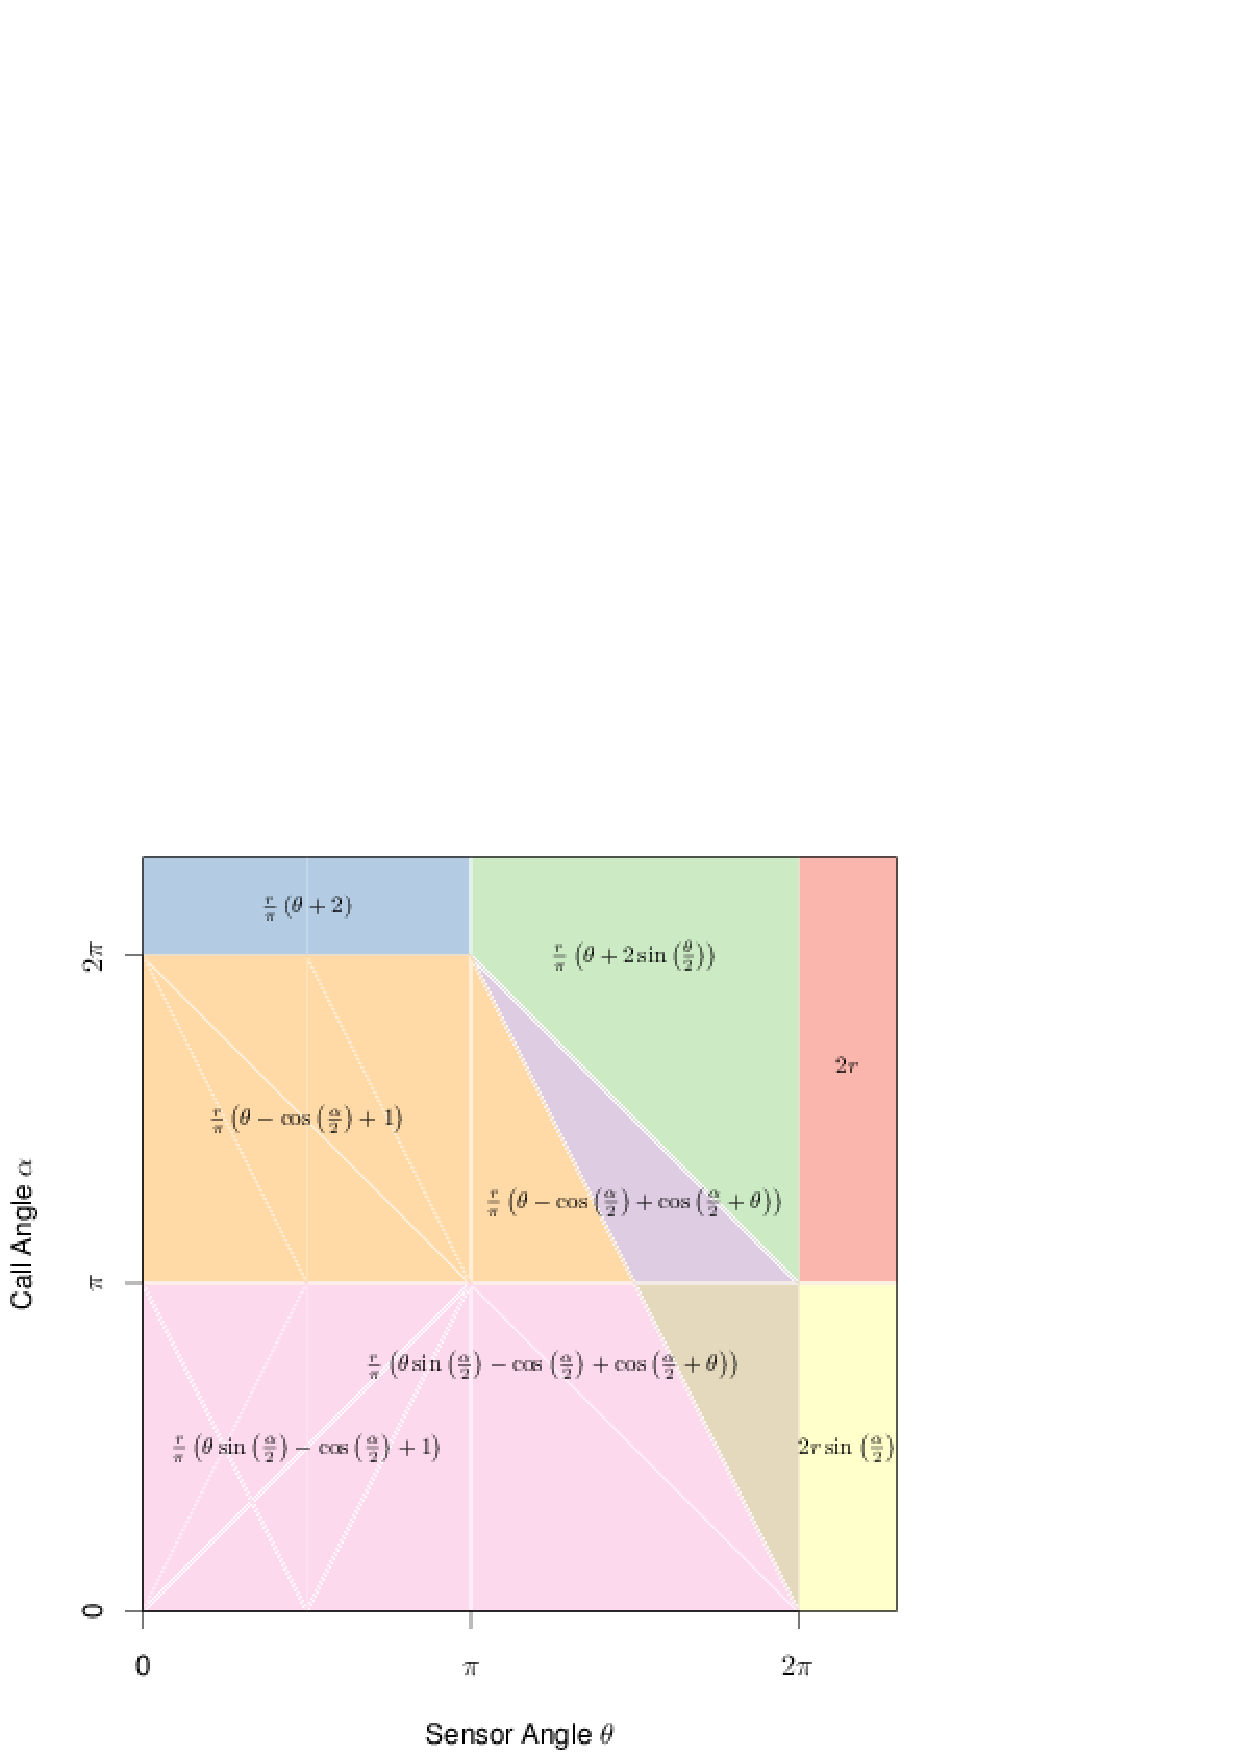
\includegraphics[width=0.6\textwidth]{imgs/equalModelResults.pdf}
\caption{Equations for the profile wide, $p$, given sensor and call widths. Each colour block represents one equation, despite independent derivation within each block, many models result in the same expression. These are collected together and presented as one block of colour.}
\label{f:equalModelResults}
\end{figure}



\subsection{Simulation model}

\begin{figure}
	\centering
	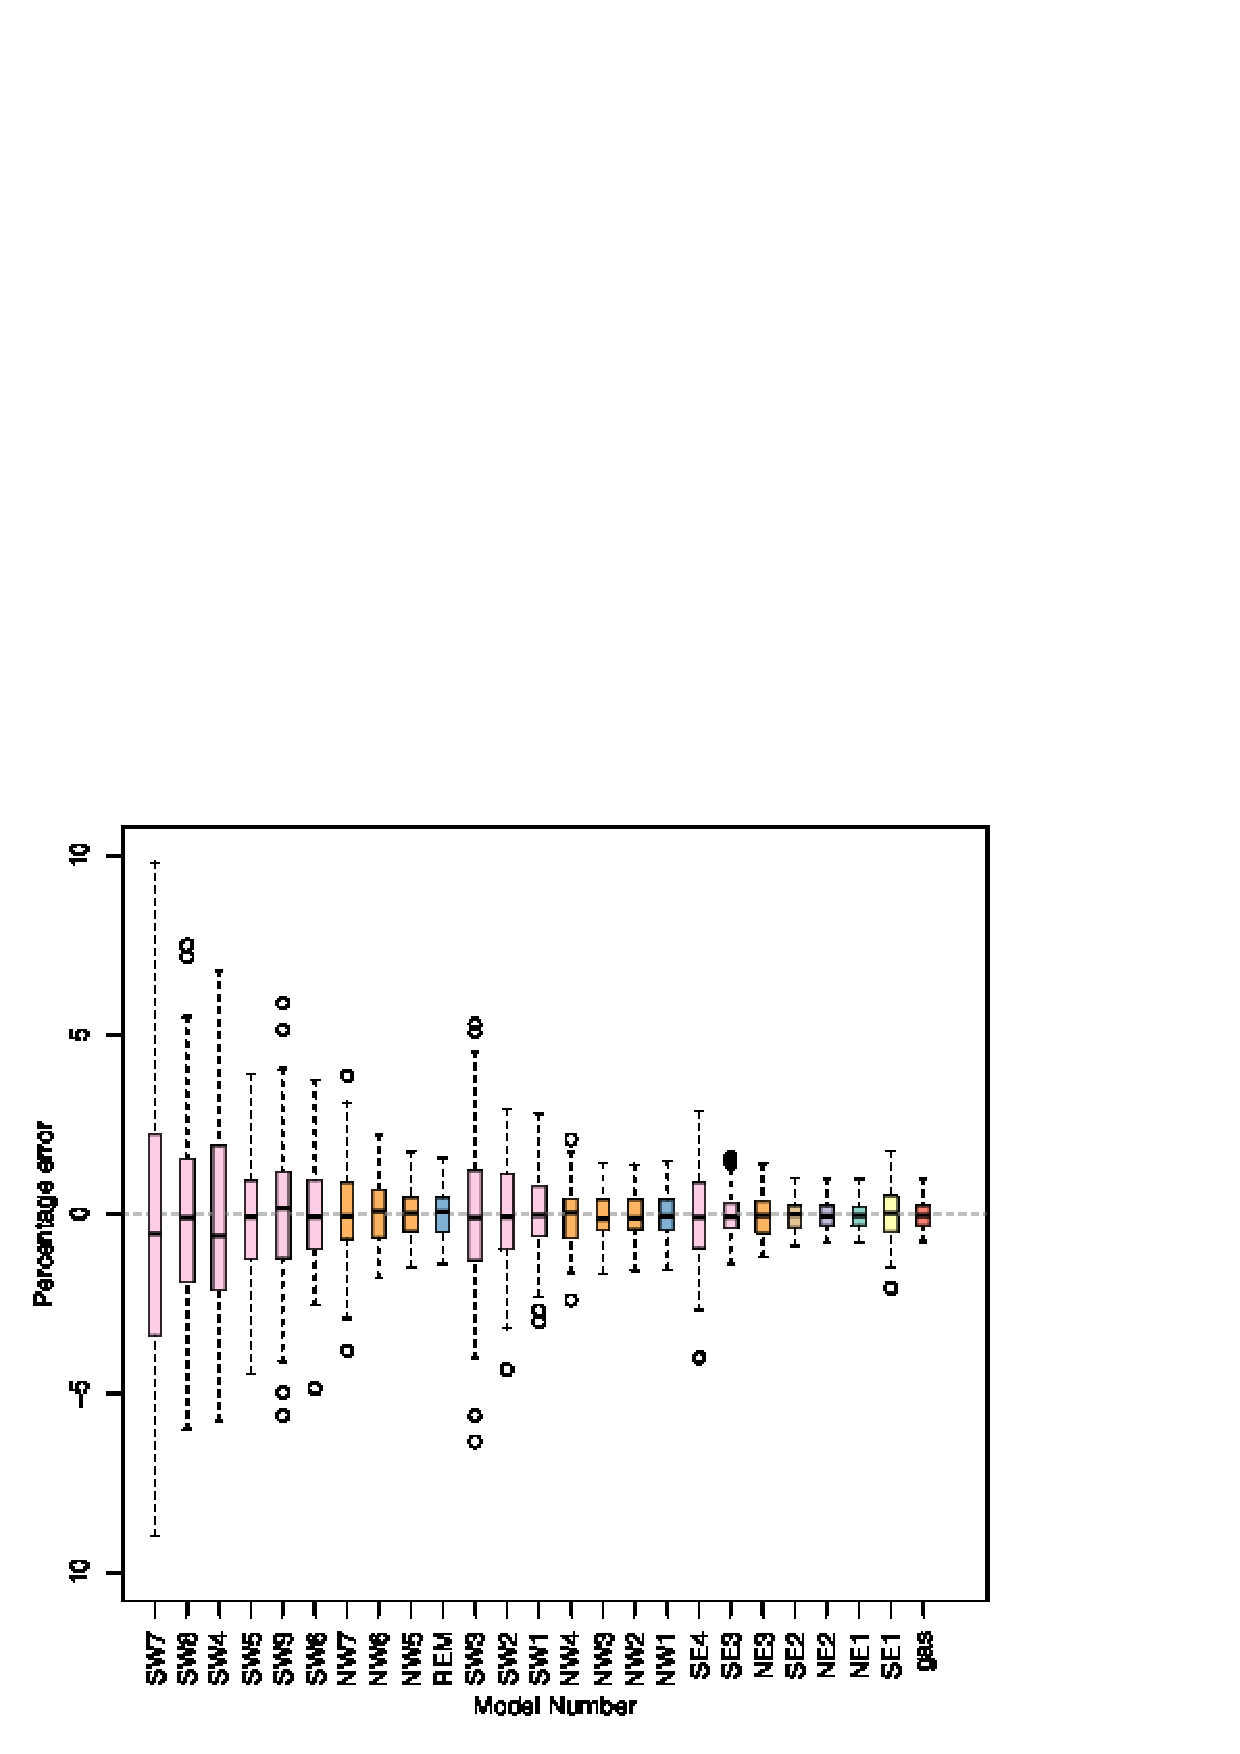
\includegraphics[width=1\textwidth]{imgs/AverageModelBias.pdf}
	\caption{Distribution of the bias for each of the derived models. Percentage error of analytical model calculated from the simulation when settings are: $r = $ \SI{100}{\meter}; $T = $ \SI{150}{\day}; $v = $ \SI{40}{\kilo\meter\per\day}; $D = $ \SI{70}{\animals\per\kilo\meter\squared}; and with detection angles varying between models. The number numbers referred to here can be found in Figure 1 Appendix S1, and the colour of each box plot match the functional form of the equation as seen in Figure~\ref{f:equalModelResults}.
  }
	\label{f:ModelBias}
\end{figure}

For each model we compared the estimated densities to the true densities in a simulation. None of the models showed any evidence of any significant differences between the estimated and true density values (Figure~\ref{f:ModelBias}). The precision of the models do vary however. The standard deviation of the error is strongly related to the call and sensor width (Figure~\ref{f:StandardDevaition}), such that larger widths have greater precision. However, even the models with small call and sensor angles have a relativity high level of precision. 

\begin{figure}[t]
        \centering
		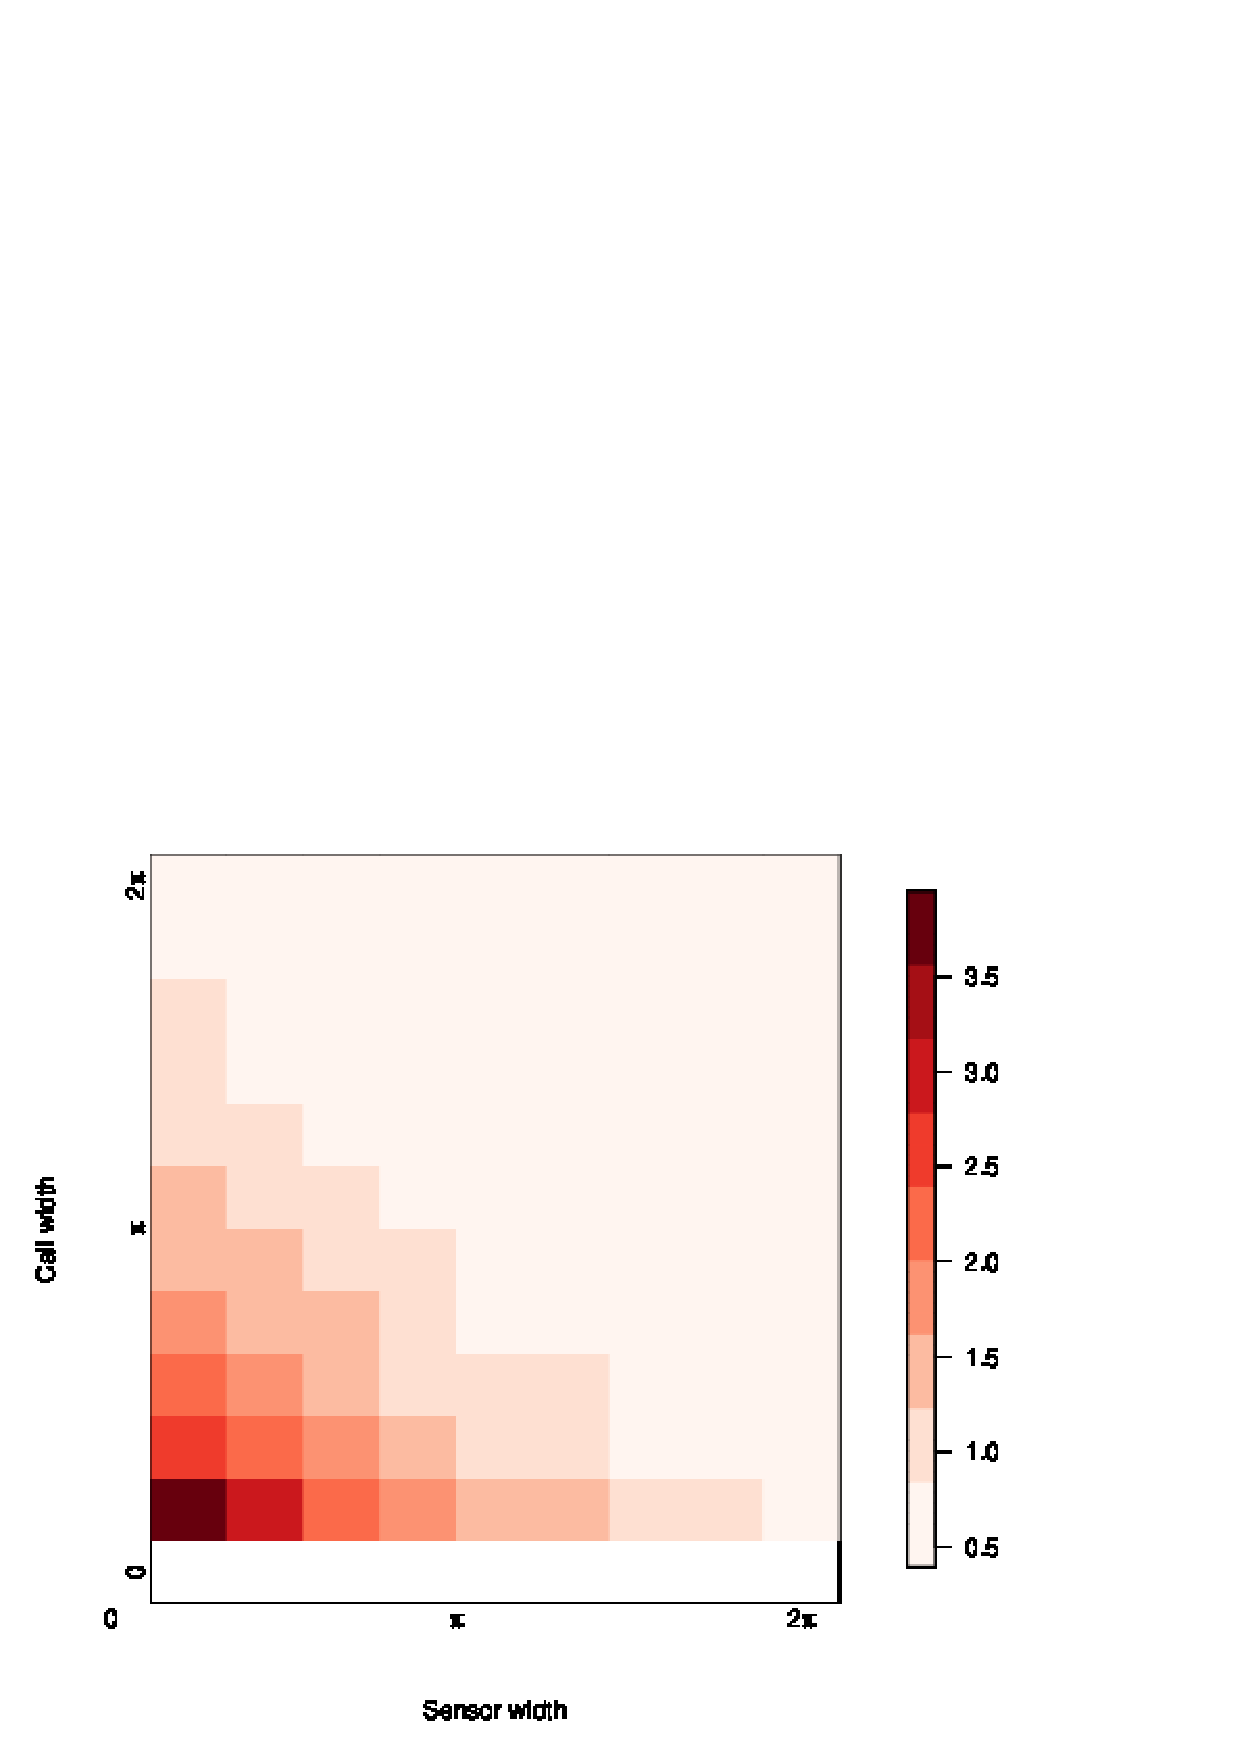
\includegraphics[width=1\textwidth]{imgs/ResultStandardDeviation.pdf}
		\caption{Angle of detector}
		\label{f:StandardDevaition}
        \caption{The precision of the gREM given a range of detection and call angles. The standard deviation of the percentage error for sensor, and call angles between 0 and $2\pi$ where: $r = $ \SI{100}{\meter}; $T = $ \SI{150}{\day}; $v = $ \SI{40}{\kilo\meter\per\day}; $D = $ \SI{70}{\animals\per\kilo\meter\squared}; and with detection angles varying between models. Where red indicates a high standard deviation and blue represents a low standard deviation.} 
\end{figure}

\begin{figure}[t]
       \centering
	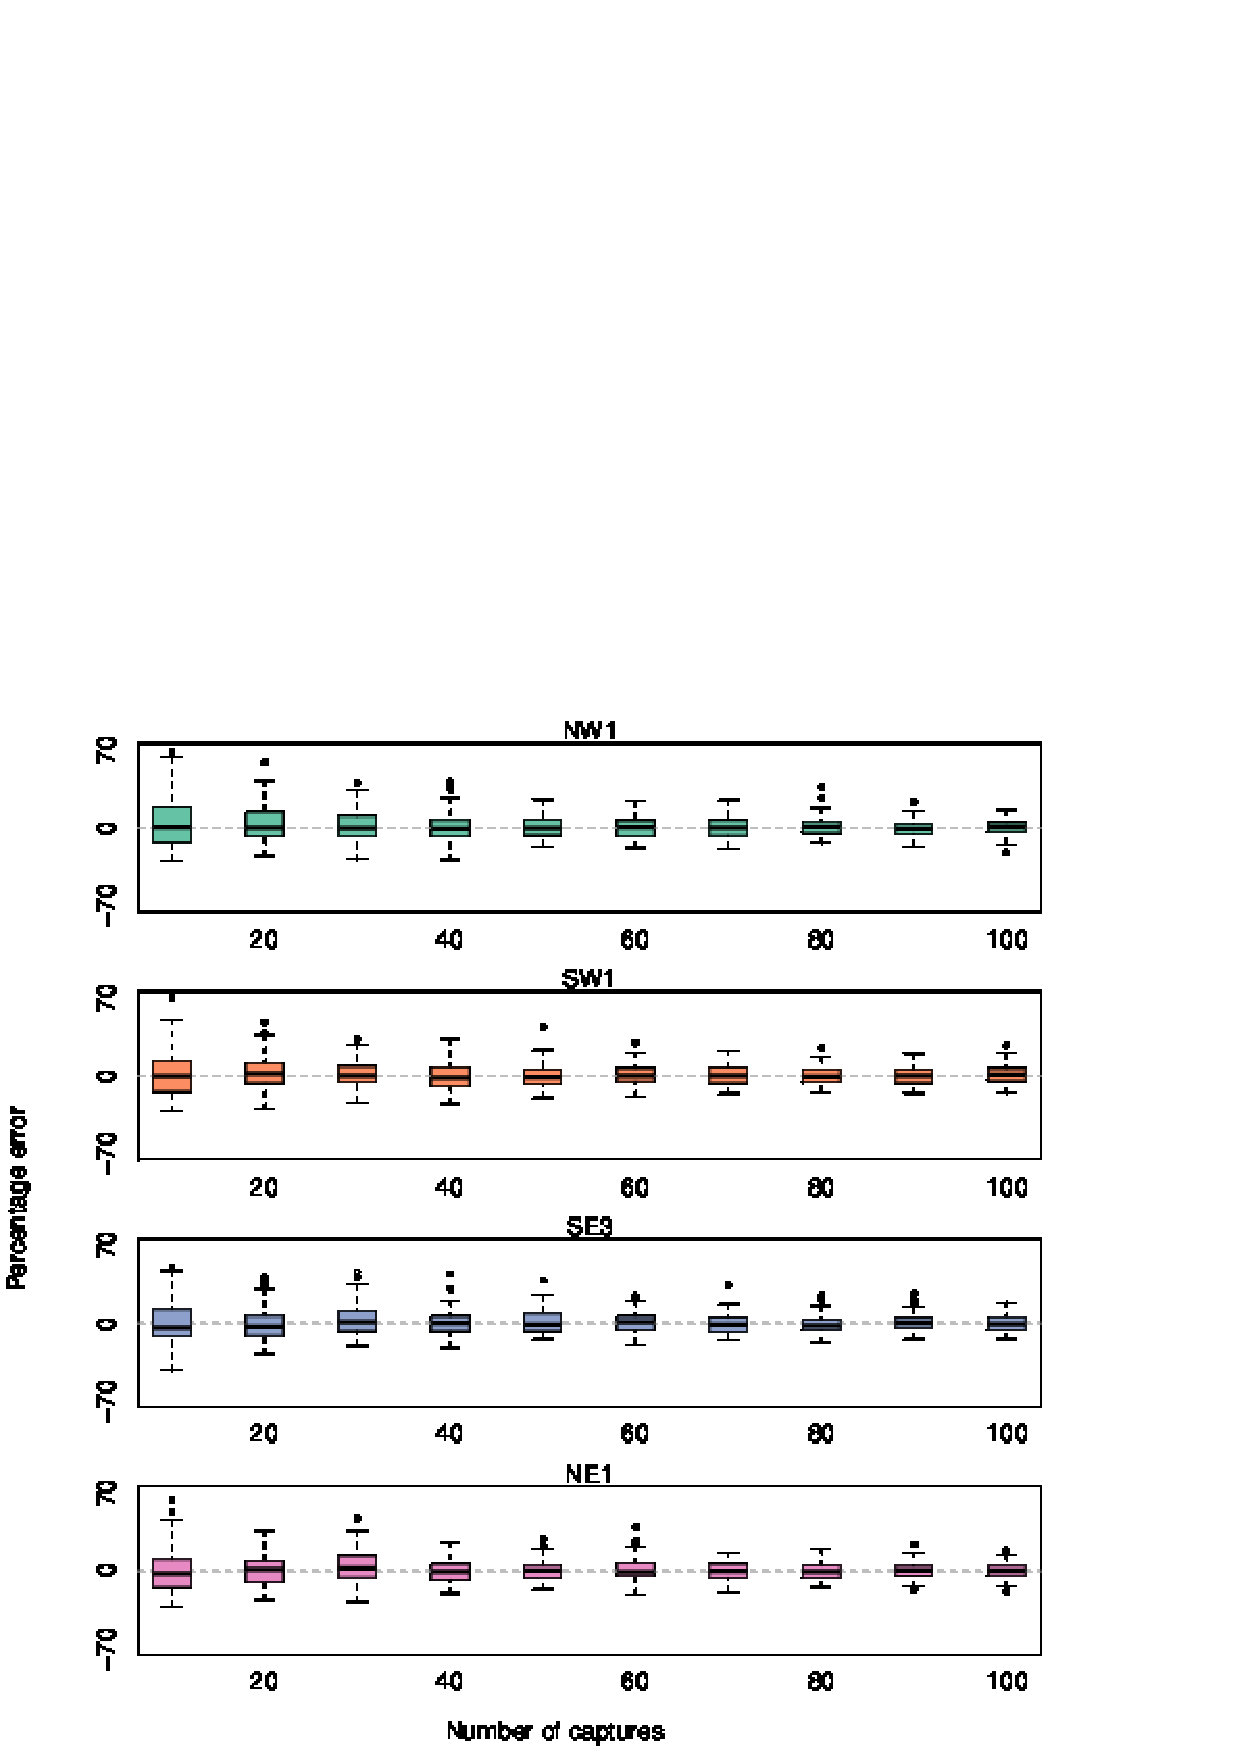
\includegraphics[width=1\textwidth]{imgs/ResultsNoCaptures.pdf}
         \caption{Number of captures}
           \label{f:Captures}
        \caption{Accuracy of the gREM reminds unchanged, whilst precision increases, with captures. Boxplots of four test models when given different numbers of captures where: $r = $ \SI{100}{\meter}; $T = $ \SI{150}{\day}; $v = $ \SI{40}{\kilo\meter\per\day}; $D = $ \SI{70}{\animals\per\kilo\meter\squared}; and with angles varying between models. Where the model names refer to Figure 1 in Appendix S1.} 
\end{figure}

The precision of the model is dependent on the number of captures during the survey. In Figure~\ref{f:Captures} we can see that the model precision gets greater as the number of captures increase. As the number of captures reaches about 100 then the coefficient of variation falls below 10\% which could be considered negligible. %The number of captures is highly dependent on the speed of the animals, the size of the detection zone, and the length of the survey, as these values increase the number of captures is also likely to increase. 

\subsubsection{Use of the gREM when animal movement is not consistent with model assumptions}

 Simulating start-stop instead of continuous movement had no effect the accuracy, or the precision, of the estimates (Figure~\ref{f:Perch}) as long as the true overall speed of the animal is known. Relaxing straight line movement to allow random or correlated random walks did not effect the accuracy of the method (Figure~\ref{f:Tort}). We allowed animals to change direction up to a maximum value at the end of each step, picked from a uniform distribution where the maximum angle ranged from 0 to $\pi$, which corresponds to straight line movement and random walk respectively. There is no significant difference in the variance for the change, this could be because of the between the step length of the animal movement, 15 minutes, means that immediate double counting of the same animal is unlikely.  In the case where large directional changes are likely to occur within short periods of time leading to double counting of the same animal within a short period of time may need to be adjusted because of this. 

\begin{figure}[t]
      \centering
	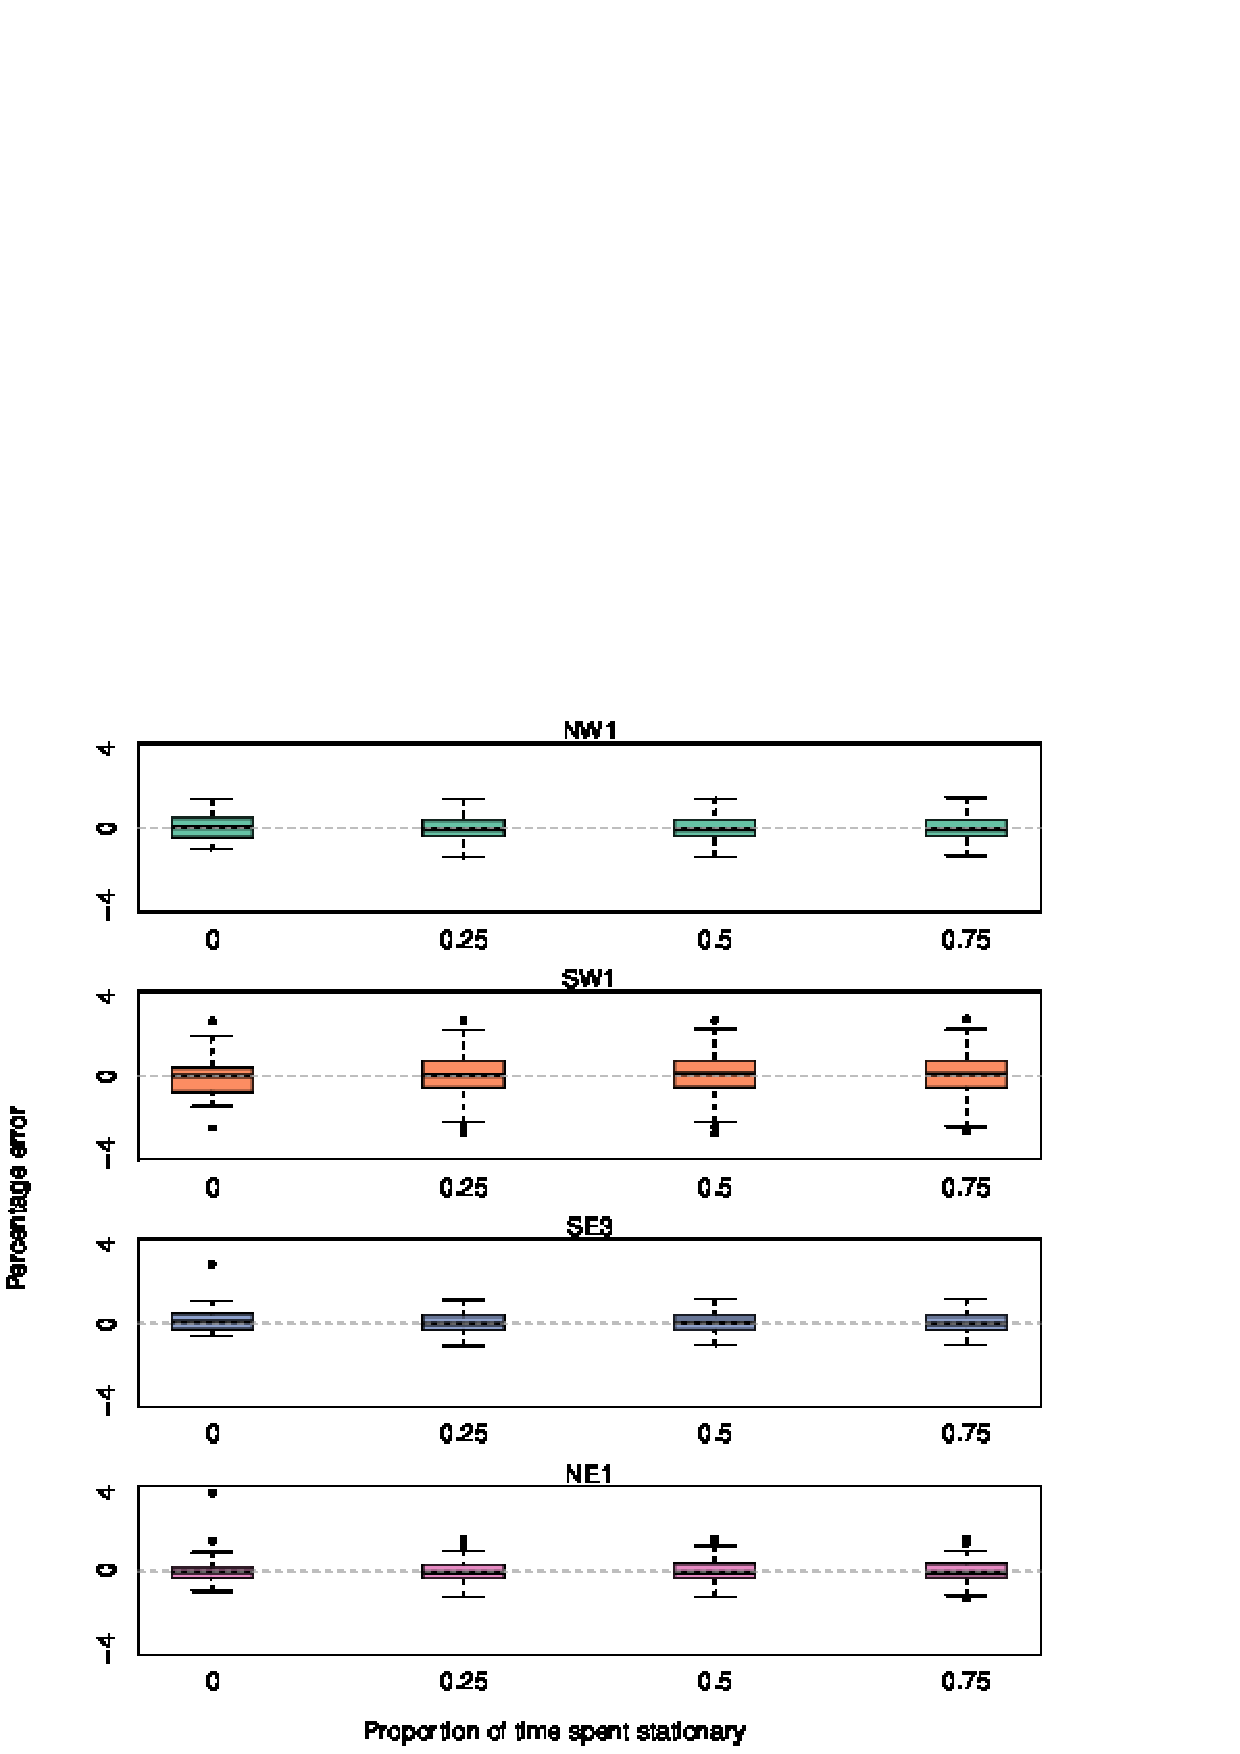
\includegraphics[width=1\textwidth]{imgs/ResultsPerch.pdf}
          \caption{Proportion of time spent stationary}
          \label{f:Perch}
	\caption{Accuracy and the precision of the gREM given changes in the amount of time an animal spends stationary on average. Distribution of model error when simulated animals spend increasing proportion of time stationary where:  $r = $ \SI{100}{\meter}; $T = $ \SI{150}{\day}; $v = $ \SI{40}{\kilo\meter\per\day}; $D = $ \SI{70}{\animals\per\kilo\meter\squared}; and with detection angles varying between models. Where the model names refer to Figure 1 in Appendix S1. } 
\end{figure}
\begin{figure}[t]
                \centering
		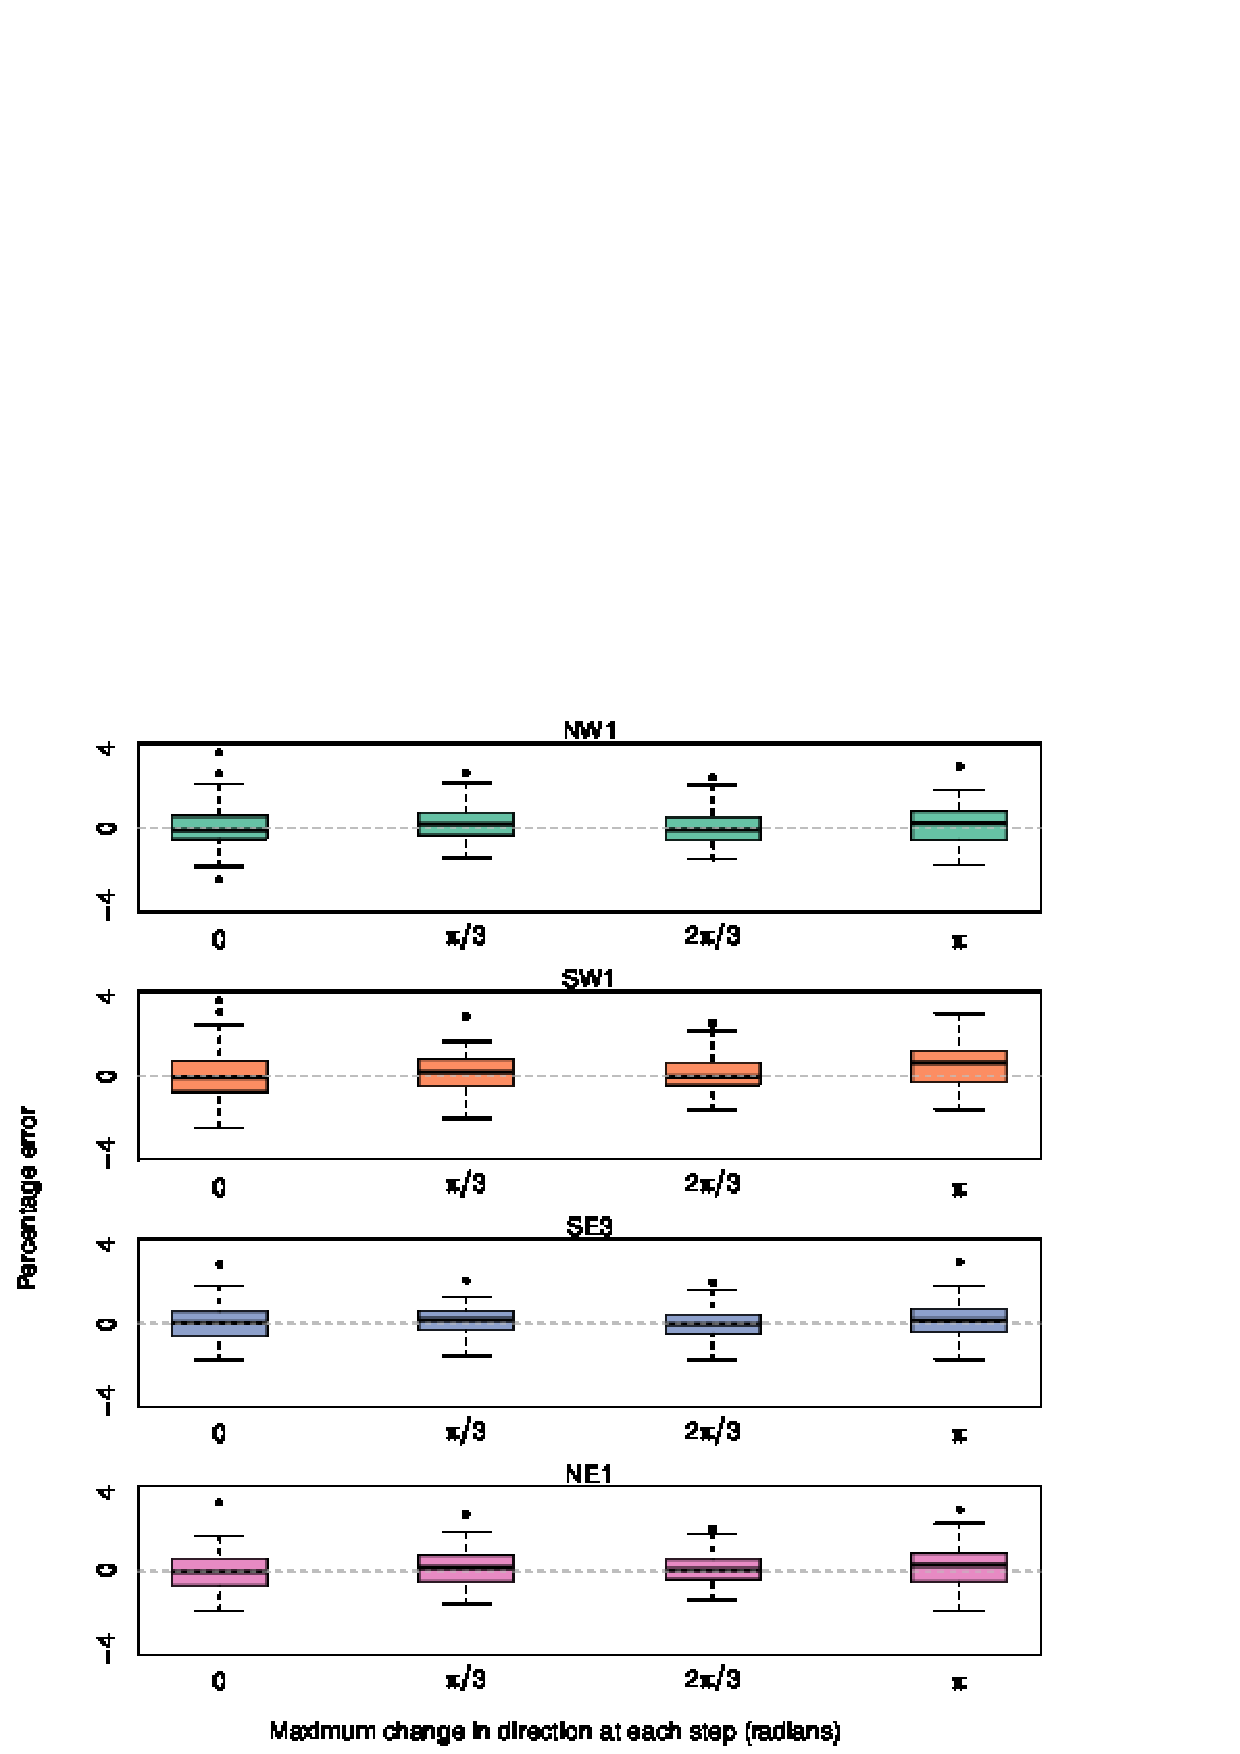
\includegraphics[width=1\textwidth]{imgs/ResultsTort.pdf}
                \caption{Angle of correlated walk}
                \label{f:Tort}
	\caption{Accuracy and the precision of the gREM given different types of correlated walks. Distribution of model error when simulated animals move with different types of correlated walk where:  $r = $ \SI{10}{\meter}; $T = $ \SI{352}{\day}; $v = $ \SI{40}{\kilo\meter\per\day}; $D = $ \SI{70}{\animals\per\kilo\meter\squared}; and with angles varying between models.Where the model names refer to Figure 1 in Appendix S1.} 
\end{figure}

                  
                  
%%%% ------- Discussion ---------%%%%
\section{Discussion}


We have developed the gREM such that it can be used to estimate density from acoustic and optical sensors. This has entailed a generalisation of the gas model and the model in \citep{rowcliffe2008estimating} to be applicable to any combination of sensor width and call directionality. We have used simulations to show, as a proof of principle, that these models are accurate and precise.

The gREM is therefore available for the estimation of density of a number of taxa of importance to conservation, zoonotic diseases and ecosystem services. The models provided are suitable for certain groups for which there are currently no, or few, effective methods for density estimation. Any species that would be consistently recorded at least once when within range of a detector would be a suitable subject for the gREM, such as bats \citep{kunz2009methods}, songbirds \citep{buckland2006point}, Cetaceans \citep{marques2009estimating} or forest primates \citep{hassel2008reliable}. Within increasing technological capabilities, this list of species is likely to increase dramatically.

Importantly the methods are noninvasive and do not require human marking or naturally identifying marks (as required for mark-recapture models). This makes them suitable for large, continuous monitoring projects with limited human resources. It also makes them suitable for species that are under pressure, species that cannot naturally be individually recognised or species that are difficult or dangerous to catch.

From our simulations  we believe that this method has the potential produce accurate and precise estimates for many different species, using either camera or acoustic detectors. When choosing detectors a researcher should pick the detector with the largest radius and detection angle possible, but whilst a small capture area may reduce precision there is only a limited impact on the overall precision of the model (Figure~\ref{f:StandardDevaition}). A range of factors will affect the overall precision of the model, like size of detection zone, speed of animal, density of animals and length of survey which are reflected in the number of captures. Increasing the number of captures leads to more precise estimates, for species which more slower, or have occur at lower densities, then the detection zone and length of survey need to be increased to compensate so that at least 100 captures are collected (Figure~\ref{f:Captures}).

Within the simulation we have assumed an equal density across the entire world, however in a field environment the situation would be much more complex, with additional variation coming from local changes in density between camera sites. We also assume perfect knowledge of the average speed of an animal and size of the detection zone, and instant triggering of the camera. All of which may lead to possible bias or decreased precision.    

Although we have used simulations to validate these models, much more robust testing is needed. Although difficult, proper field test validation would be required before the models could be fully trusted. Note, however, that the REM \citep{rowcliffe2008estimating} has been field tested. Both \citet{rowcliffe2008estimating} and \citet{zero2013monitoring} both found that the REM were effective manner of estimating animal densities \citep{rowcliffe2008estimating, zero2013monitoring}. There was some discrepancies between the REM and the census methodologies found by Rovero and Marshall which may have been down to lack of knowledge of wild animal speed, and an underestimate in census results \citep{rovero2009camera}. In some taxa gold standard methods of estimating animal density exist, such as capture mark recapture. Where these gold standard exist, and have been proved to work, a simultaneous gREM study could be completed to test the accuracy under field conditions. An easier way to continue to evaluate the models is to run more extensive simulations which break the assumptions of the analytical models. The main element that cannot be analytically treated is the complex movement of real animals. Therefore testing these methods against true animal traces, or more complex movement models would be useful.


There are a number of positive extensions to the gREM which could be developed in the future. The original gas model was formulated for the case where both subjects, either animal and detector, or animal and animal, are moving \citep{Hutchinson_Waser_2007}. Indeed any of the models with animals that are equally detectable in all directions ($\alpha = 2\pi$) can be trivially expanded for moving by substituting the sum of the average animal velocity and the sensor velocity for $v$ as used here. However, when the animal has a directional call, the extension becomes much less simple. The approach would be to calculate again the mean profile width. However, for each angle of approach, one would have to average the profile width for an animal facing in any direction (i.e. not necessarily moving towards the sensor) weighted by the relative velocity of that direction. There are a number of situations where a moving detector and animal could occur and as such may be advantage to have a method of estimating densities from the data collected, e.g. an acoustic detector based off a boat when studying Cetacea or sea birds \citep{yack2013passive}.

Another interesting, and so far unstudied problem, is edge effects caused by trigger delays (the delay between sensing an animal and attempting to record the encounter) and time expansion acoustic detectors which repeatedly turn on an off during sampling. Both of these have potential biases as animals can move through the detection zone without being detected. The models herein are formulated assuming constant surveillance and so the error quickly becomes negligible. For example, if it takes longer for the recording device to be switched on than the length of some animal calls there could be a systematic underestimation of density. 

%%%% ------- Acknowledgments ---------%%%%
\section{Acknowledgments}



\bibliographystyle{mee.bst}	
\bibliography{lucas-moorcroft-etal-refs.bib}	

\end{document}
		

